\documentclass[letterpaper,11pt]{article}
\oddsidemargin -1.0cm \textwidth 17.5cm

\usepackage[utf8]{inputenc}
\usepackage[activeacute,spanish]{babel}
\usepackage{amsfonts,setspace}
\usepackage{amsmath}
\usepackage{amssymb, amsmath, amsthm}
\usepackage{comment}
\usepackage{amssymb}
\usepackage{dsfont}
\usepackage{anysize}
\usepackage{multicol}
\usepackage{enumerate}
\usepackage{graphicx}
\usepackage[left=1.5cm,top=2cm,right=1.5cm, bottom=1.7cm]{geometry}
\setlength\headheight{1.5em} 
\usepackage{fancyhdr}
\usepackage{multicol}
\usepackage{hyperref}
\usepackage{wrapfig}
\pagestyle{fancy}
\fancyhf{}
\renewcommand{\labelenumi}{\normalsize\bfseries P\arabic{enumi}.}
\renewcommand{\labelenumii}{\normalsize\bfseries (\alph{enumii})}
\renewcommand{\labelenumiii}{\normalsize\bfseries \roman{enumiii})}

\begin{document}

\fancyhead[L]{\itshape{Facultad de Ciencias F\'isicas y Matem\'aticas}}
\fancyhead[R]{\itshape{Universidad de Chile}}

\begin{minipage}{11.5cm}
    \begin{flushleft}
        \hspace*{-0.6cm}\textbf{FI1000-5 Introducción a la Física Clásica}\\
        \hspace*{-0.6cm}\textbf{Profesora:} Paulina Lira\\
        \hspace*{-0.6cm}\textbf{Auxiliares:} Alejandro Silva, Juan Cristóbal Castro\\
    \end{flushleft}
\end{minipage}

\begin{picture}(2,3)
    \put(405,-5){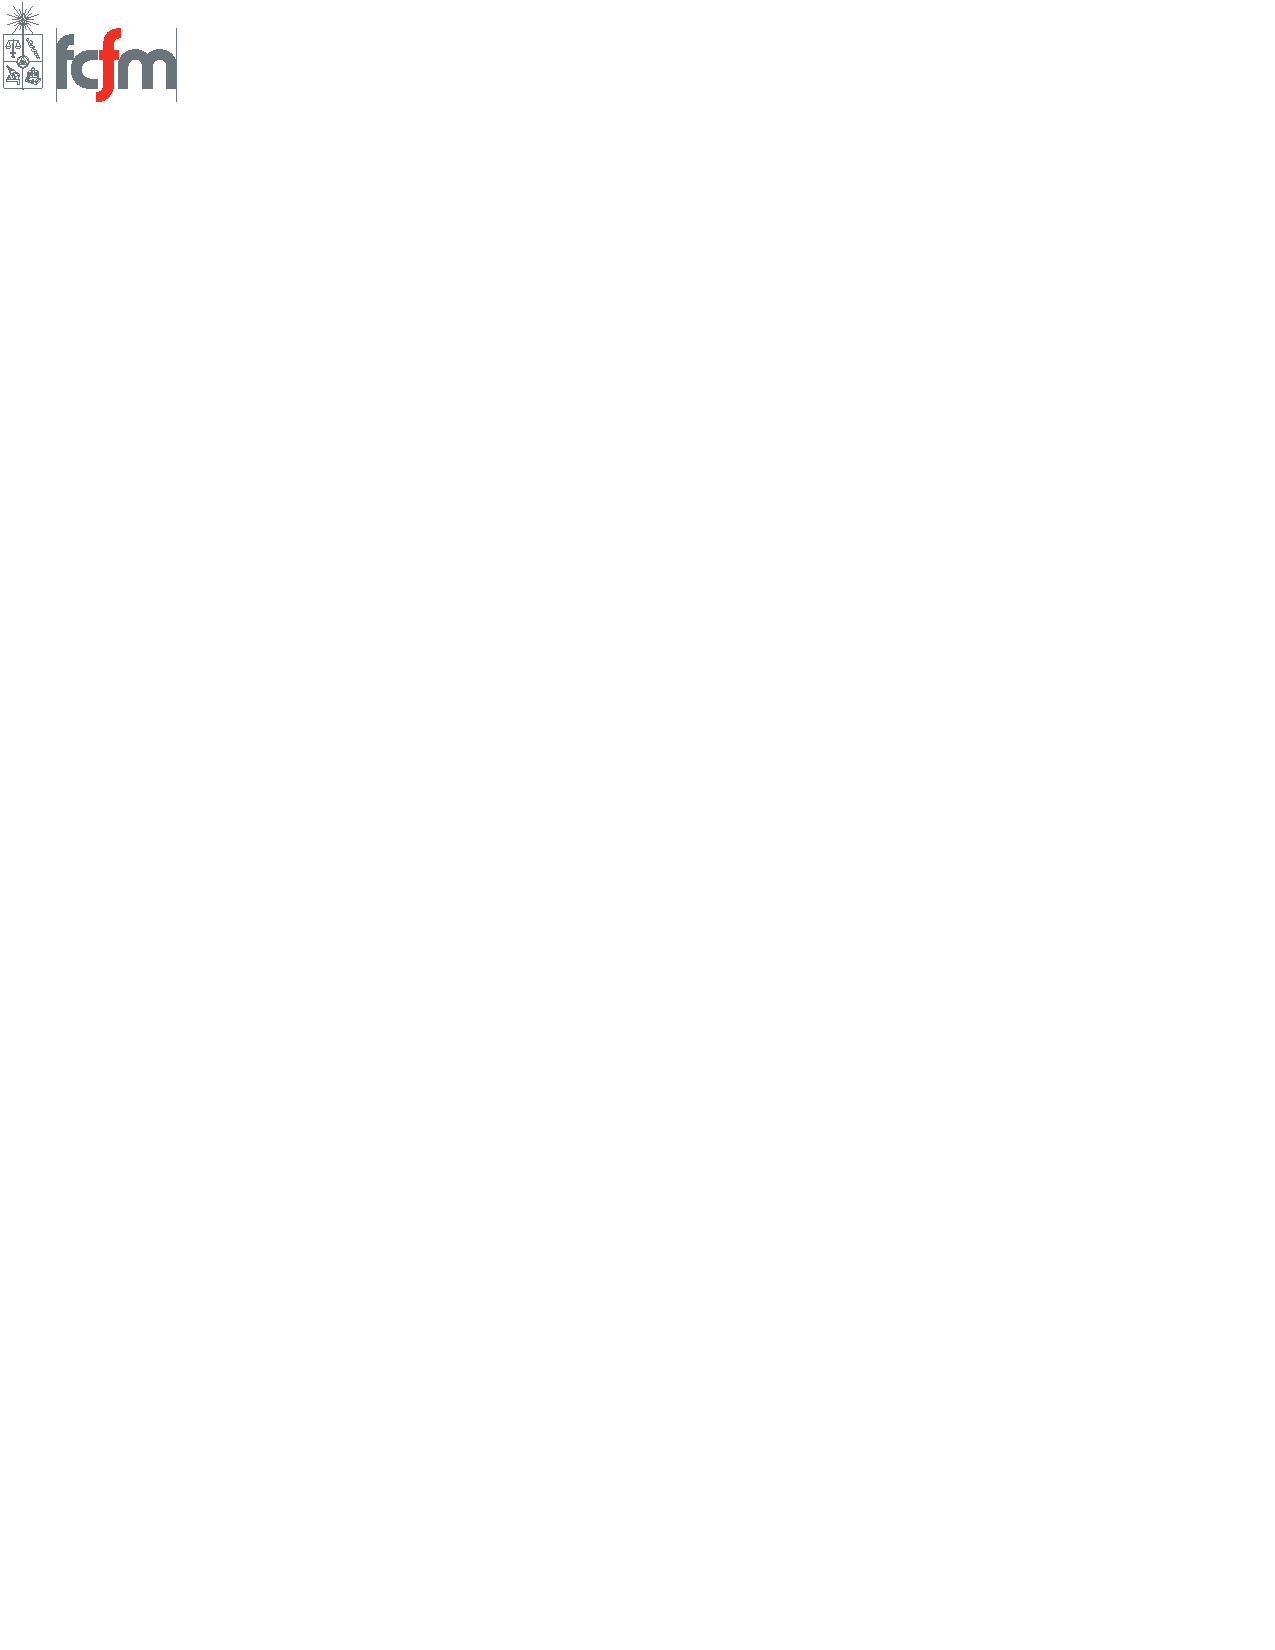
\includegraphics[scale=1.25]{2020-1/Imágenes/logo/fcfm2.pdf}}
\end{picture}

\begin{center}
	\LARGE \bf Auxiliar 7   \\
\end{center}

\vspace{-0,5cm}
\begin{enumerate}\setlength{\itemsep}{0.4cm}

\rfoot[]{pág. \thepage}

\item Una bloque de masa m se posa sobre una cuña. Por un lado se conecta con una superficie fija mediante una cuerda ideal. La cuerda es tensada gracias a la acción de la masa colgante M. Por el otro lado, el bloque, se encuentra sujeto a un resorte de constantes k, $l_0$.\\
\begin{figure}[h!]
    \centering
    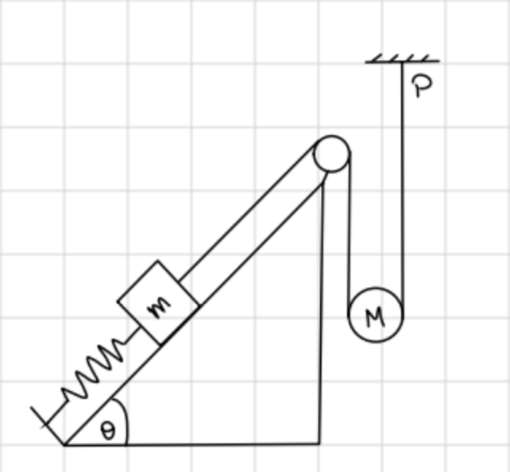
\includegraphics[scale = 0.3]{2020-1/Imágenes/aux8/1.png}
\end{figure}
\begin{enumerate}
    \item Encuentre una razón entre las masas m y M para que el resorte trabaje a tracción y a comprensión. Suponga $\theta$ conocido.
    \item Encuentre $\theta$ tal que el sistema se mantenga en equilibrio
\end{enumerate}

\item Una caja de masa M es sostenida por dos resortes idénticos de constantes k, $l_0$. El sistema se dispone verticalmente en presencia de gravedad como se muestra en la figura. La separación entre los puntos A y B es tal que cuando el bloque se dispone en el punto medio, ninguno de los resortes experimenta elongación. Dentro de la caja se posa una moneda de masa m. Sabiendo que el sistema se encuentra en equilibrio, determine la distancia máxima que se puede subir el bloque tal que al soltarlo la moneda no se separe de la caja.
\begin{figure}[h!]
    \centering
    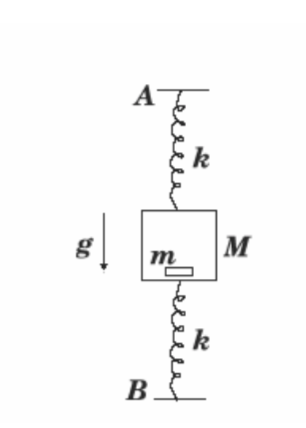
\includegraphics[scale = 0.5]{2020-1/Imágenes/aux8/2.png}
\end{figure}
\end{enumerate}
\end{document}